\section{Distanz-Testaufbau}
Der Sensor wurde auf einem Breadboard mit einem Arduino Uno verbunden und übertrug die Werte
via USB-Kabel an den Seriellen Monitor der Arduino IDE. Um eine mögliche Schieflage auf dem
Breadboard abzufedern wurden aus 200 Messungen der Durchschnitt berechnet und von den Werten vor
der Verarbeitung subtrahiert. So liegt der Sensor mathematisch flach auf. \\

\subsection{Distanzmessungen}
Insgesamt wurden 10 Tests pro Formel gemacht, die Ergebnisse können Sie unten einsehen.\\

\begin{figure} [h]
    \centering
    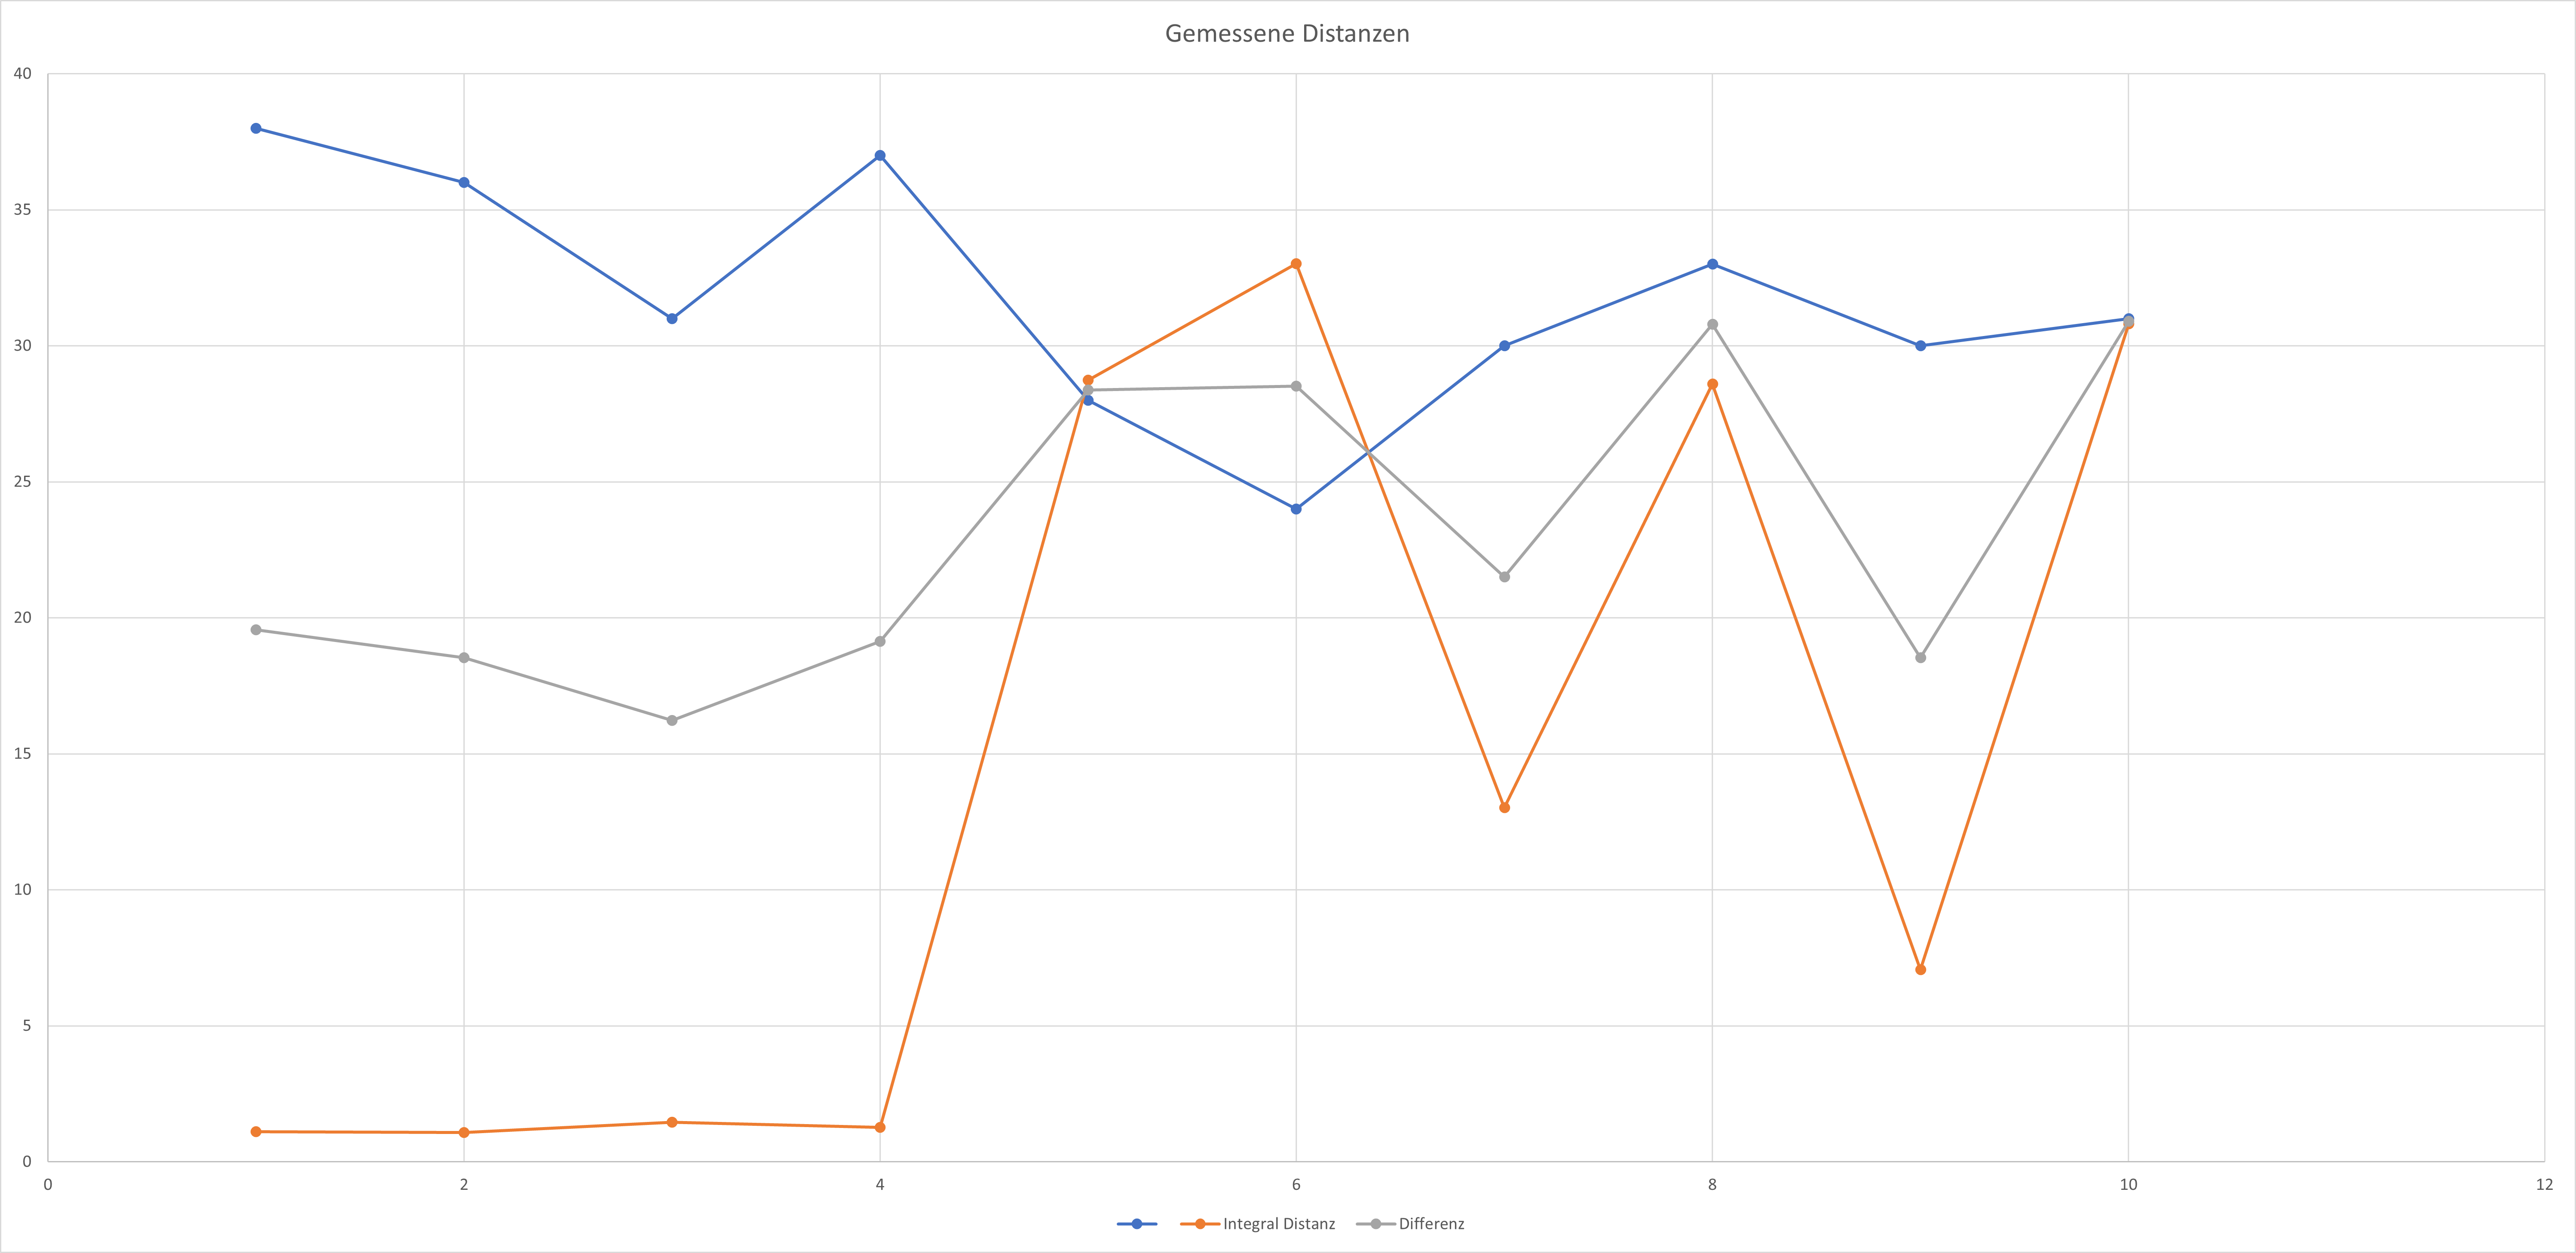
\includegraphics[width = 15cm]{Bilder/_DistanzVergleich}
    \caption{Distanzen | Alle Tests}
    %\label{fig:wo-bin-ich}
    \end{figure}

\subsection{Fehler}
Die zwei weiteren Graphen zeigen die Fehler bei 10 sek"undigem Stillstand. Der exponentielle Drift 
bei der Integralen Formel ist typisch. 

\begin{figure} [h]
    \centering
    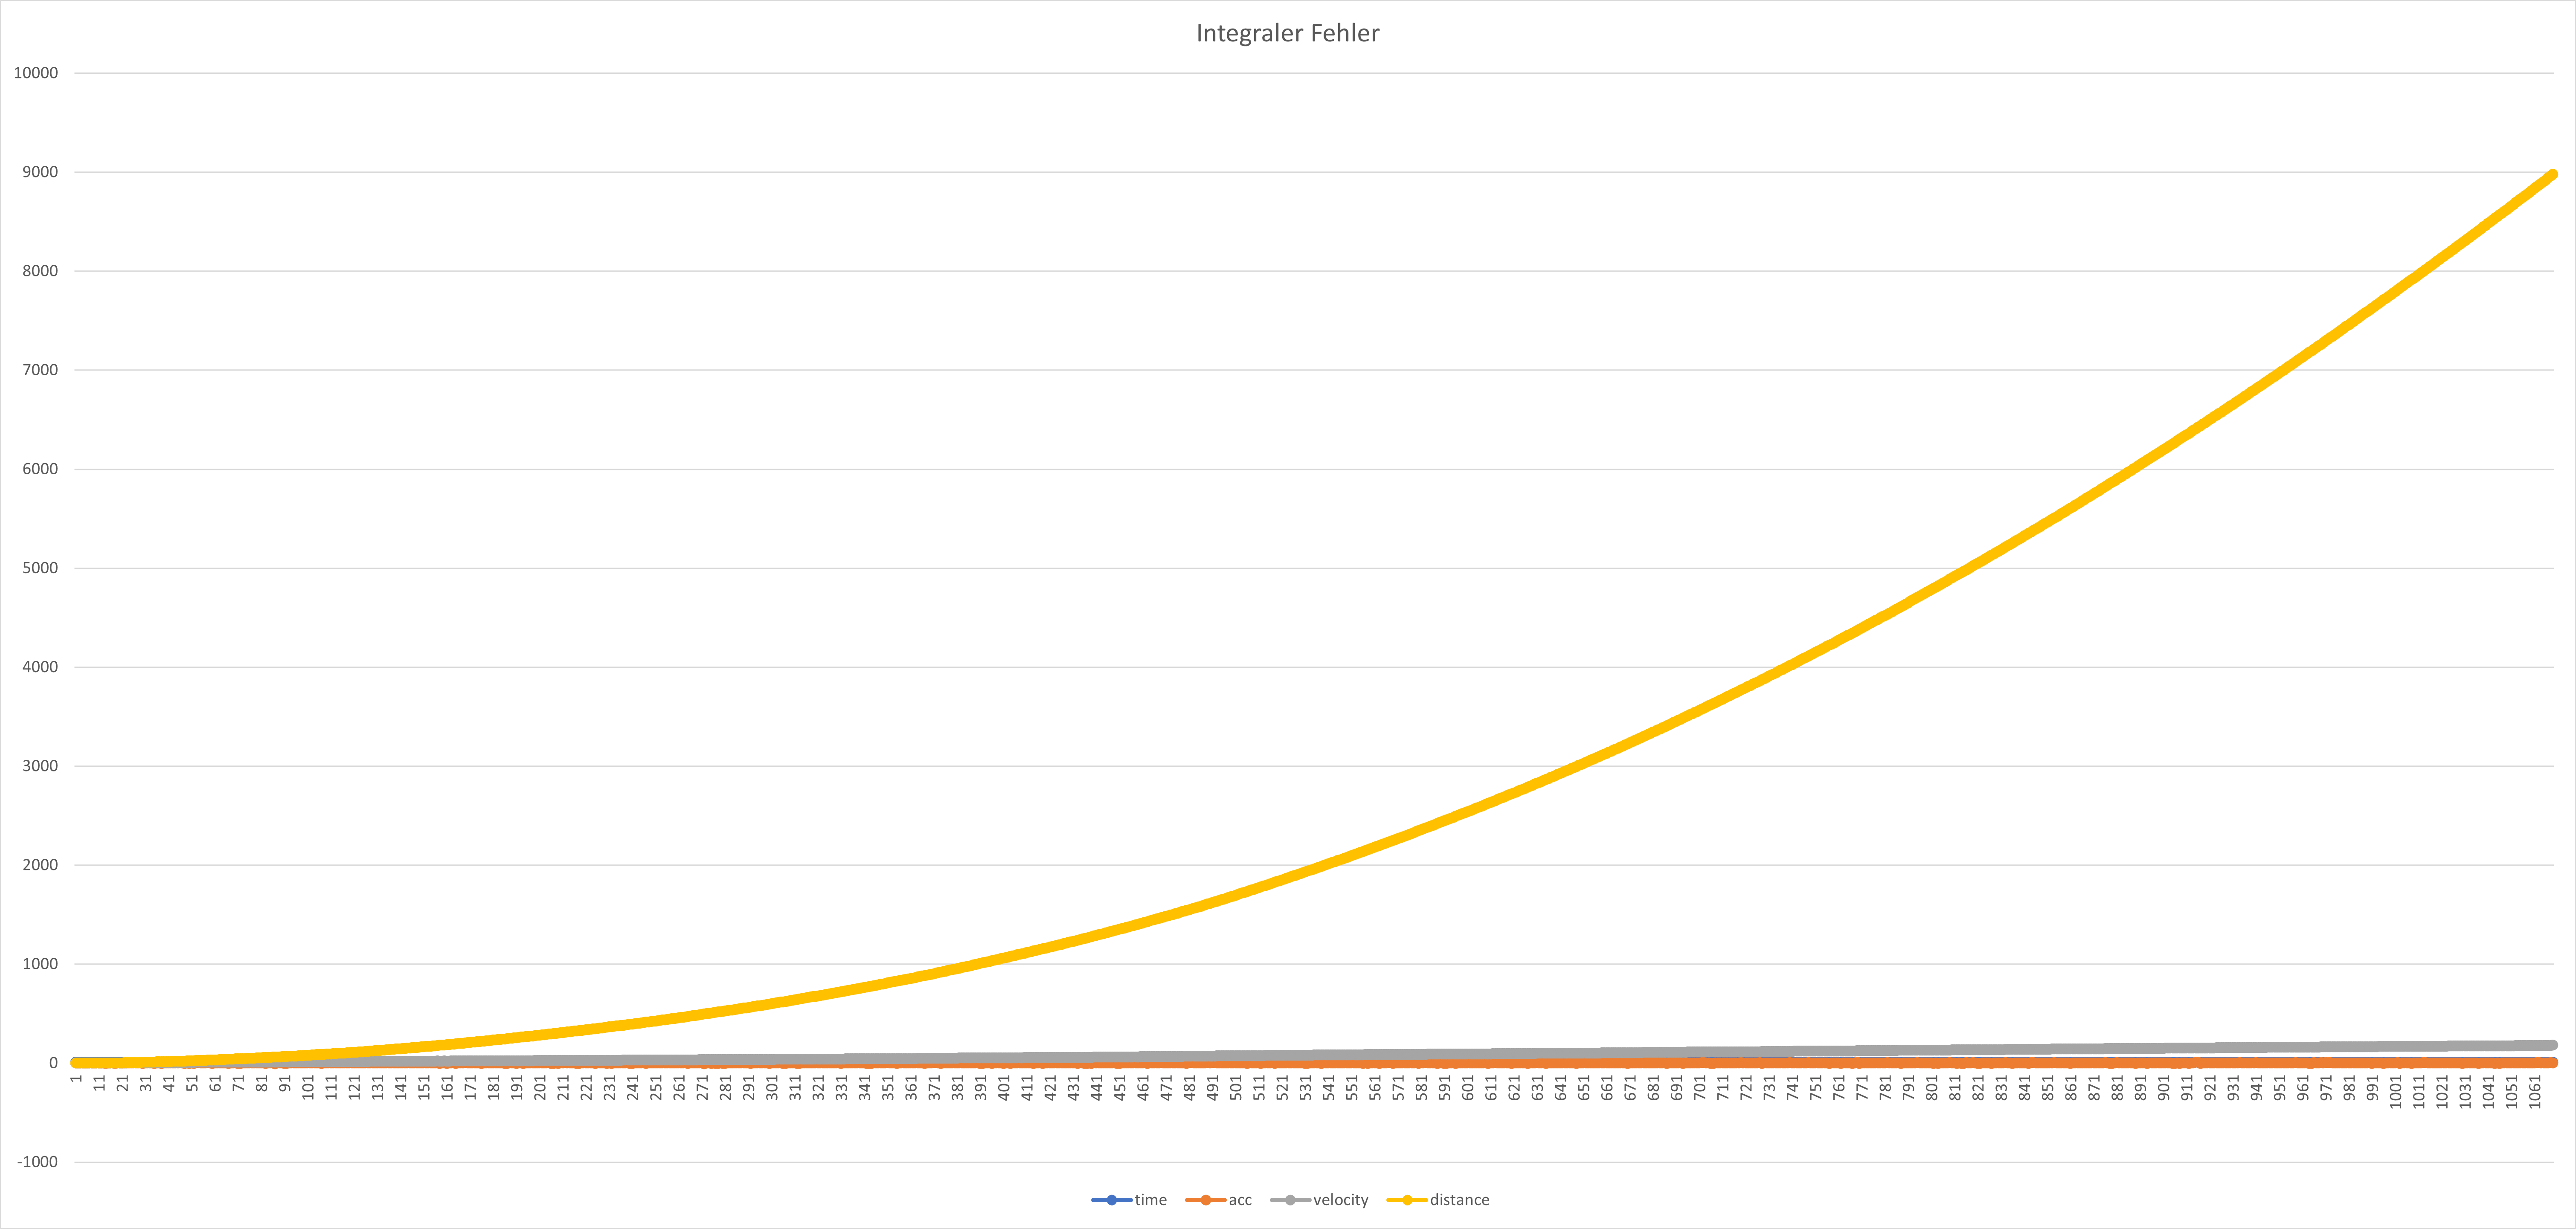
\includegraphics[width = 15cm]{Bilder/_integralDistance001}
    \caption{Integrale Formel | Drift}
    %\label{fig:wo-bin-ich}
    \end{figure}

    \begin{figure} [h]
        \centering
        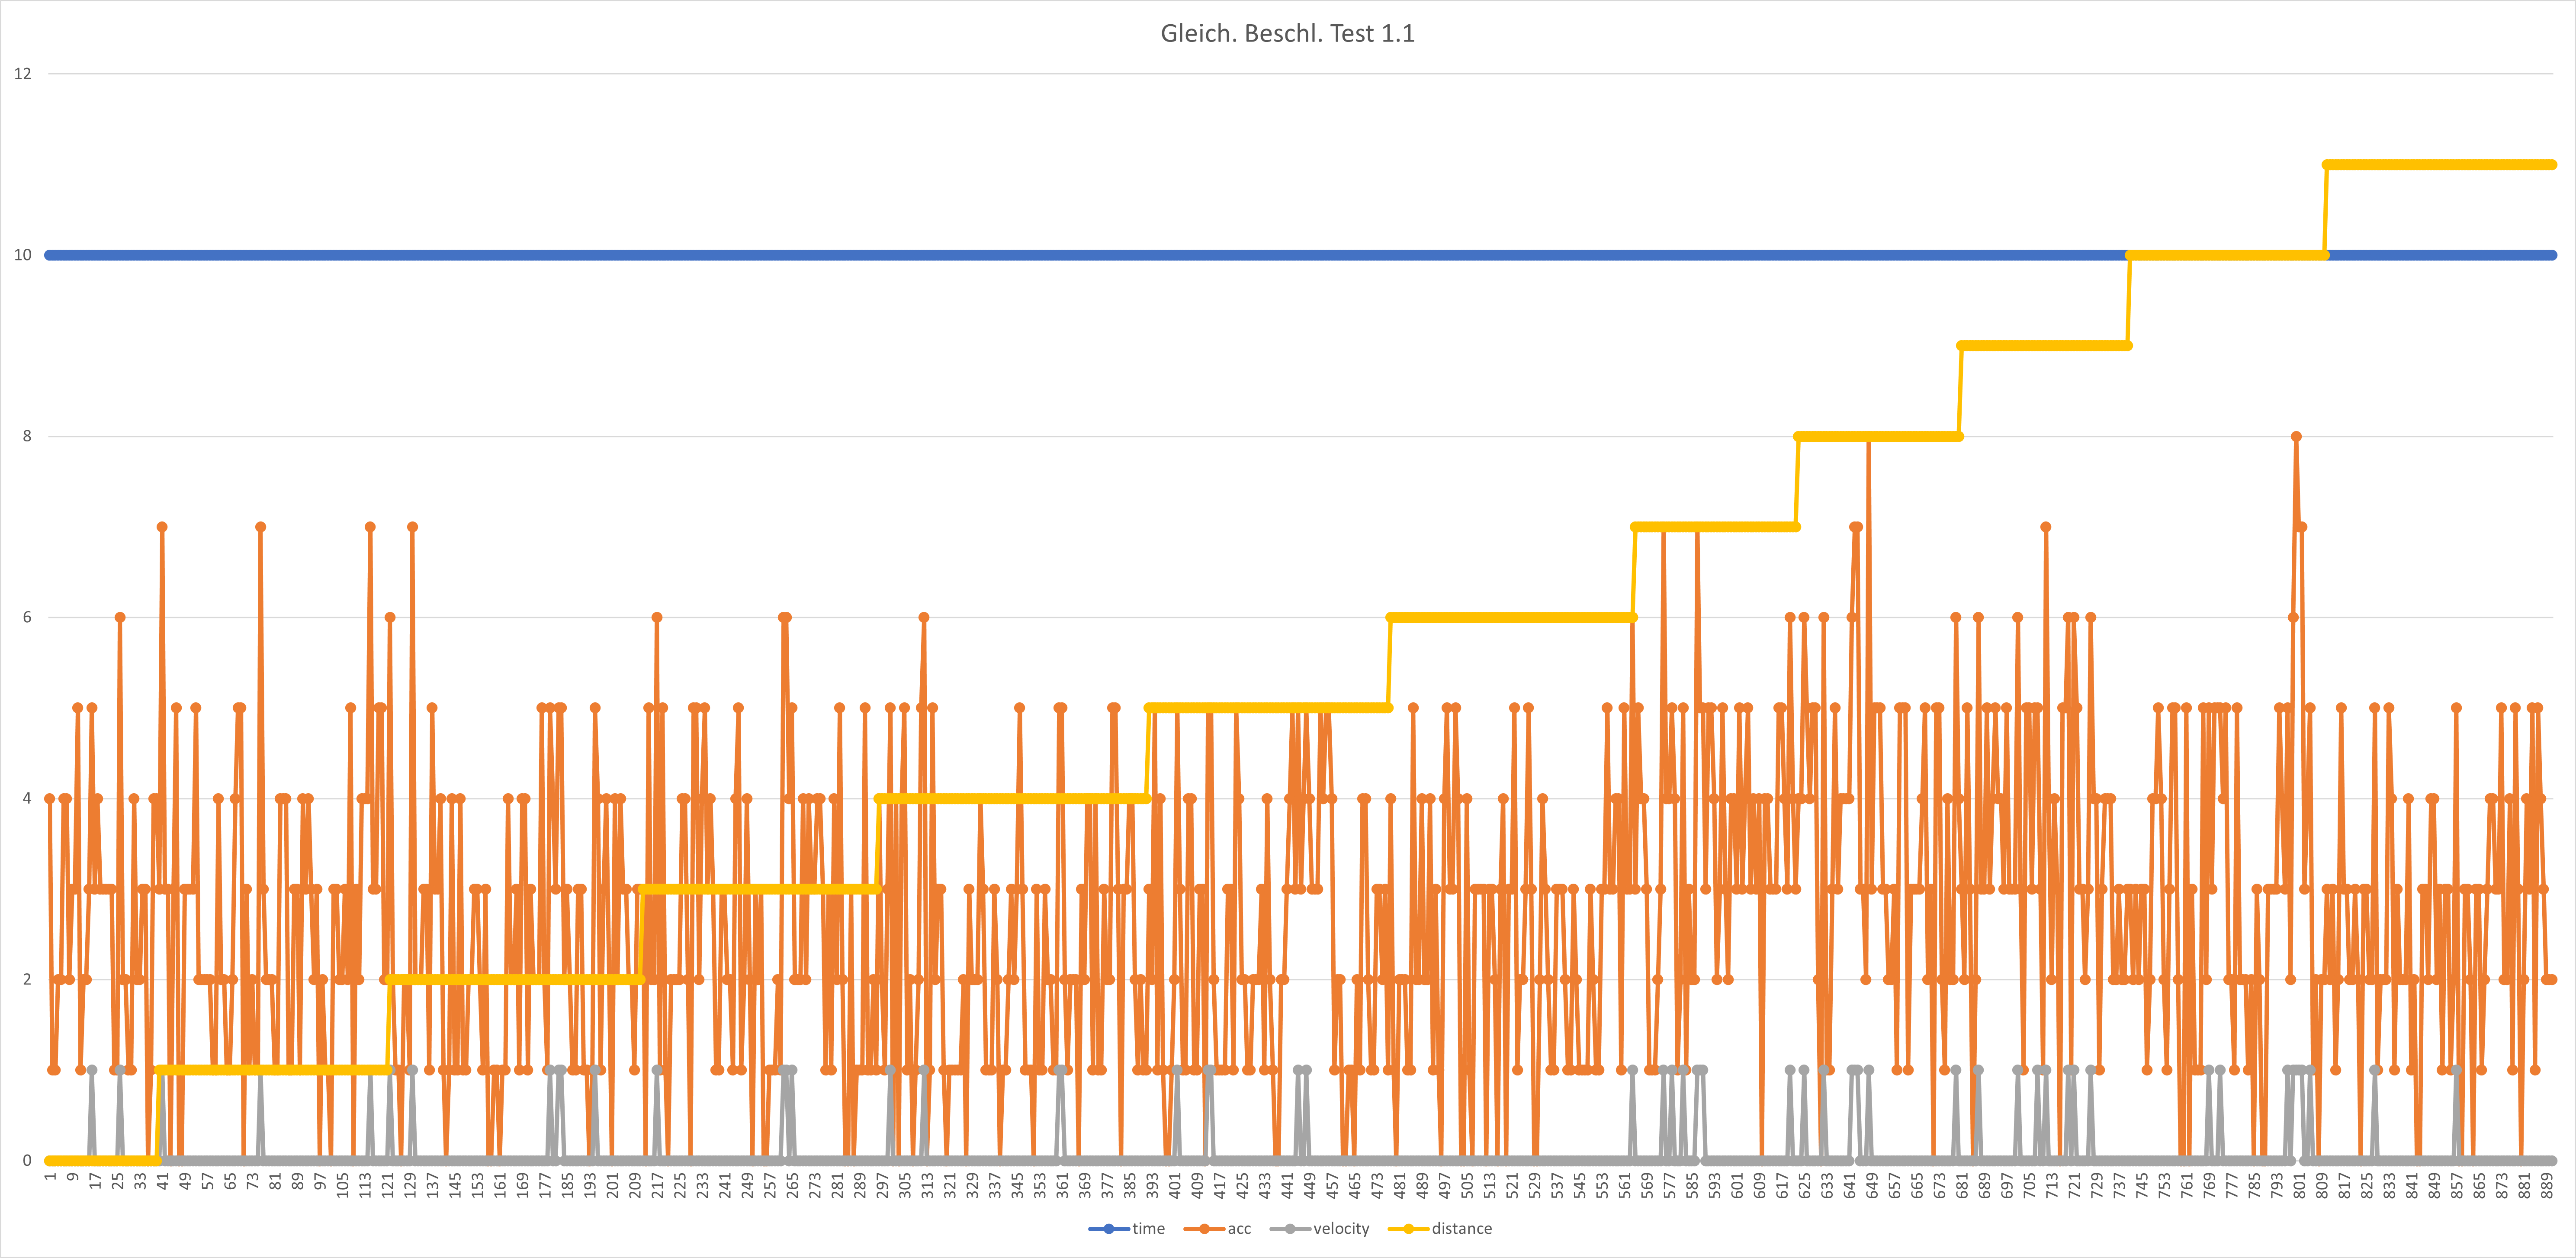
\includegraphics[width = 15cm]{Bilder/_constDistance001}
        \caption{Gleichf"ormige Beschl. Formel | Drift}
        %\label{fig:wo-bin-ich}
        \end{figure}
    
Auch die Fehler in den Distanzmessungen sind zu groß, als das 
eine zuverlässige, über auch nur Minuten gehende Distanzberechnung für mein Projektziel sinnvoll wäre.